\documentclass[submit]{harvardml}

\course{CS181-S20}
\assignment{Assignment \#5}
\duedate{11:59pm April 10, 2020} 
\newcommand{\attr}[1]{\textsf{#1}}
\usepackage[OT1]{fontenc}
\usepackage[colorlinks,citecolor=blue,urlcolor=blue]{hyperref}
\usepackage[pdftex]{graphicx}
\usepackage{subfig}
\usepackage{fullpage}
\usepackage{amsmath}
\usepackage{amssymb}
\usepackage{color}
\usepackage{todonotes}
\usepackage{listings}
\usepackage{common}
\usepackage{bm}
\usepackage{enumitem}
\usepackage{tikz}
\usepackage{xifthen}
\usepackage{soul}

\usepackage[mmddyyyy,hhmmss]{datetime}

\definecolor{verbgray}{gray}{0.9}

\lstnewenvironment{csv}{
  \lstset{backgroundcolor=\color{verbgray},
  frame=single,
  framerule=0pt,
  basicstyle=\ttfamily,
  columns=fullflexible}}{}

\begin{document}
\begin{center}
{\Large Homework 5: Mixtures, EM, and Graphical Models}\\
\end{center}

This homework assignment will have you work with mixtures, EM, and
graphical models.  

Please type your solutions after the corresponding problems using this
\LaTeX\ template, and start each problem on a new page.

Please submit the \textbf{writeup PDF to the Gradescope assignment `HW5'}. Remember to assign pages for each question.

Please submit your \textbf{\LaTeX\ file and code files to the Gradescope assignment `HW5 - Supplemental'}. 

You can use a \textbf{maximum of 2 late days} on this assignment.  Late days will be counted based on the latest of your submissions. 
\\

\begin{problem}[Expectation-Maximization for Categorical-Geometric Mixture Models, 25pts]

In this problem we will explore expectation-maximization for a
Categorical-Geometric Mixture model.  Each observation $\boldx_n$ is a
positive integer scalar drawn from a geometric distribution
(associated with the number of trials needed to get to the first
success, if success occurs with probability $p$).  We posit that each
observation comes from \emph{one} mixture component.  For this
problem, we will assume there are $K$~components. Each component $k
\in \{1, \ldots, K\}$ will be associated with a probability $p_k \in
    [0,1]$.  Finally let the (unknown) overall mixing proportion of
    the components be~$\btheta \in [0,1]^K$, where~${\sum_{k=1}^K
      \btheta_k=1}$.

Our generative model is that each of the~$N$ observations comes from a
single component.  We encode observation $n$'s component-assignment as
a one-hot vector~${\boldz_n \in \{0,1\}^K}$ over components. This
one-hot vector is drawn from~$\btheta$; then, $\boldx_n$ is drawn
from~$\text{Geometric}(p_k )$ where $\boldx_n$ belongs to class $k$.

Formally, data are generated in two steps (assuming $\boldz_n$ encodes
the class $k$), where we define the PMF of the geometric distribution to be $p(x_n | p_k) = (1 - p_k)^{x_n - 1} p_k$:
\begin{eqnarray*}
 \boldz_n &\sim& \text{Categorical}(\btheta) \\
 \boldx_n &\sim& \text{Geometric}(p_k )
\end{eqnarray*}

  \begin{enumerate}

  \item \textbf{Intractability of the Data Likelihood} We are
    generally interested in finding a set of parameters $p_k$ that
    maximize the data likelihood $\log
    p(\{\boldx_n\}^N_{n=1}|\{p_k\}^K_{k = 1})$.  Expand the data
    likelihood to include the necessary sums over observations
    $\boldx_n$ and latents $\boldz_n$.  Why is optimizing this loss
    directly intractable?

\item \textbf{Complete-Data Log Likelihood} Define the complete data
  for this problem to be $D = \{(\boldx_n, \boldz_n)\}_{n=1}^N$. Write
  out the complete-data negative log likelihood. Note that optimizing
  this loss is now computationally tractable if we know $\boldz_n$.

\[\mcL(\btheta, \{p_k\}^K_{k=1}) =  -\ln p(D \given\btheta, \{p_k\}^K_{k=1}).\]


\item \textbf{Expectation Step} Our next step is to introduce a
  mathematical expression for $\boldq_n$, the posterior over the
  hidden topic variables~$\boldz_n$ conditioned on the observed data
  $\boldx_n$ with fixed parameters, i.e $p(\boldz_n | \boldx_n;
  \btheta, \{ p_k \}^K_{k=1})$.

\begin{itemize}
\item  \textbf{Part 3.A } Write down and simplify the expression for $\boldq_n$.
\item  \textbf{Part 3.B } Give an algorithm for calculating the expression for $\boldq_n$ found in Part 3.A for all $n$, given the observed data~$\{\boldx_n\}^N_{n=1}$ and settings of the parameters~$\btheta$ and~$\{ p_k\}^K_{k=1}$.

\end{itemize}

\item \textbf{Maximization Step}
Using the~$\boldq_n$ estimates from the Expectation Step, derive an update for maximizing the expected complete data log likelihood in terms of~$\btheta$ and~$\{ p_k \}^K_{k=1}$.

\begin{itemize}
    \item \textbf{Part 4.A } Derive an expression for the expected complete-data log likelihood using $\boldq_n$.
    \item \textbf{Part 4.B } Find an expression for $\btheta$ that maximizes this expected complete-data log likelihood. You may find it helpful to use Lagrange multipliers in order to enforce the constraint $\sum \btheta_k = 1$. Why does this optimized $\btheta$ make intuitive sense?
    \item \textbf{Part 4.C } Apply a similar argument to find the
      values of $\{p_k \}^K_{k = 1}$ that maximizes the expected
      complete-data log likelihood.
\end{itemize}

\item Suppose that this had been a classification problem. That is,
  you were provided the ``true'' categories $\boldz_n$ for each observation $\boldx_n$,
  and you were going to perform the classification by
  inverting the provided generative model (i.e. now you're predicting $z$ given $x$). Could you reuse any of
  your inference derivations above?

\item Finally, implement your solution (see \texttt{T5\_P1.py} for starter code).  You are responsible for implementing the \texttt{loglikelihood}, \texttt{e\_step} and \texttt{m\_step} functions. Test it out with data given
  $10$ samples from $3$ components with $p_1 = .1$, $p_2=.5$, and
  $p_3=.9$.  How does it perform?  What if you increase the number of
  samples to $1000$ from each of the components?  What if you change
  $p_2=.2$?  Hypothesize reasons for the differences in performance
  when you make these changes. You may need to record five to ten trials (random restarts) in order to observe meaningful insights.

\end{enumerate}

\end{problem}

\subsection*{Solution}
\begin{enumerate}
    \item 
        \begin{equation*}
            p(\{\boldx_n\}^N_{n=1}|\{p_k\}^K_{k = 1})
        \end{equation*}
        \begin{equation*}
             p(\{\boldx_n\}^N_{n=1}|\{p_k\}^K_{k = 1}) = \sum_{i=1}^K p(x_n, z_n = i | \{p_k\}^K_{k = 1})
        \end{equation*}
        \begin{equation*}
             p(\{\boldx_n\}^N_{n=1}|\{p_k\}^K_{k = 1}) = \sum_{i=1}^K p(x_n | z_n = i, \{p_k\}^K_{k = 1}) p(z_n = i)
        \end{equation*}
        \begin{center}
            We are given that $p(z_n = i) = \btheta_i$
        \end{center}
        \begin{equation*}
             p(\{\boldx_n\}^N_{n=1}|\{p_k\}^K_{k = 1}) = \sum_{i=1}^K p(x_n | z_n = i, \{p_k\}^K_{k = 1}) \btheta_{i}
        \end{equation*}
        \begin{center}
            We are given that $x_n|z_n$ comes from Geom$(p_{z_n})$ and we can apply the PMF.
        \end{center}
        \begin{equation*}
            p(\{\boldx_n\}^N_{n=1}|\{p_k\}^K_{k = 1}) = \sum_{i=1}^K (1-p_i)^{x_n - 1}p_i \btheta_{i}
        \end{equation*}
        \begin{center}
            Now we have all N data points
        \end{center}
        \begin{equation*}
            p(\{\boldx_n\}^N_{n=1}|\{p_k\}^K_{k = 1}) = \prod_{j = 1}^N\sum_{i=1}^K (1-p_i)^{x_j - 1}p_i \btheta_{i}
        \end{equation*}
        \begin{center}
            Lastly, we take the log
        \end{center}
        \begin{equation*}
            \log p(\{\boldx_n\}^N_{n=1}|\{p_k\}^K_{k = 1}) = \sum_{j = 1}^N\log(\sum_{i=1}^K (1-p_i)^{x_j - 1}p_i \btheta_{i})
        \end{equation*}
        
        By trying to optimize this loss, we have to sum the $K$ classes over of the latent variable $\boldz_{n}$ is inside of a log which means we cannot get a closed form solution. This is because consolidating a summation inside of a log is not possible.
    
    \item
        \begin{equation*}
            p(D \given\btheta, \{p_k\}^K_{k=1}) =  p(\{(\boldx_n, \boldz_n)\}_{n=1}^N \given\btheta, \{p_k\}^K_{k=1})
        \end{equation*}
        \begin{equation*}
            p(D \given\btheta, \{p_k\}^K_{k=1})  =  \prod_{j=1}^N p(x_j, z_j \given\btheta, \{p_k\}^K_{k=1})
        \end{equation*}
        \begin{equation*}
            p(D \given\btheta, \{p_k\}^K_{k=1})  =  \prod_{j=1}^N p(x_j \given z_j,\btheta, \{p_k\}^K_{k=1}) p(z_j \given\btheta, \{p_k\}^K_{k=1})
        \end{equation*}
        \begin{equation*}
            p(D \given\btheta, \{p_k\}^K_{k=1}) = \prod_{j=1}^N (1-p_{z_j})^{x_j - 1}p_{z_j} \btheta_{z_j}
        \end{equation*}
        \begin{center}
            Now we take the negative log
        \end{center}
        \begin{equation*}
             \mcL(\btheta, \{p_k\}^K_{k=1}) = - \log \prod_{j=1}^N (1-p_{z_j})^{x_j - 1}p_{z_j} \btheta_{z_j}
        \end{equation*}
        \begin{equation*}
             \mcL(\btheta, \{p_k\}^K_{k=1}) = - \sum_{j=1}^N \log ((1-p_{z_j})^{x_j - 1}p_{z_j} \btheta_{z_j})
        \end{equation*}
        \begin{equation*}
             \mcL(\btheta, \{p_k\}^K_{k=1}) = - \sum_{i=1}^K\sum_{j=1}^N z_{ij} \log ((1-p_{i})^{x_j - 1}p_{i} \btheta_{i})
        \end{equation*}
        \begin{equation*}
             \mcL(\btheta, \{p_k\}^K_{k=1}) = - \sum_{i=1}^K\sum_{j=1}^N z_{ij} ((x_j -1) \log(1 - p_i) + \log(p_i) + \log(\btheta_{i}))
        \end{equation*}
    
    \item
        \textbf{Part 3.A }
        \begin{equation*}
            \boldq_{n} = p(\boldz_n | \boldx_n; \btheta, \{ p_k \}^K_{k=1})
        \end{equation*}
        \begin{equation*}
            \boldq_{n} = \frac{p(\boldz_n, \boldx_n; \btheta, \{ p_k \}^K_{k=1})}{p(\boldx_n; \btheta, \{ p_k \}^K_{k=1})}
        \end{equation*}
        \begin{center}
            Now we want this, but for a single $n$ point
        \end{center}
        \begin{equation*}
            \boldq_{n} = \frac{(1-p_{z_n})^{x_n - 1}p_{z_n} \btheta_{z_n}}{\sum_{k =1}^K (1-p_{k})^{x_n - 1}p_{k} \btheta_{k}}
        \end{equation*}
    
        \textbf{Part 3.B }\newline
        Each $j$-th element of $\boldq_n$ can be represented by $p(\boldz_n = j\given \boldx_n; \btheta, \{ p_k \}^K_{k=1})$. So,
            \begin{equation*}
                p(\boldz_n = j\given \boldx_n; \btheta, \{ p_k \}^K_{k=1}) = \frac{(1-p_{j})^{x_n - 1}p_{j} \btheta_{j}}{\sum_{k = 1}^K (1-p_{k})^{x_n - 1}p_{k} \btheta_{k}}
            \end{equation*}
        This is for a single data point for all $j \in \{1, ... , K\}$, so we want to calculate these values and then store them in a $1 \times K$ vector. We then want to do this for all $N$ data points and store those as subsequent rows. So we will end up with a $N\times K$ where each row represents the $\boldq_n$ of a specific point.
        
    \item
        \textbf{Part 4.A }\newline
        We take the result from part 2
        \begin{equation*}
            \mcL(\btheta, \{p_k\}^K_{k=1}) = - \sum_{i=1}^K\sum_{j=1}^N z_{ij} ((x_j -1) \log(1 - p_i) + \log(p_i) + \log(\btheta_{i}))
        \end{equation*}
        And then take the expectation
        \begin{equation*}
            \mathbb{E}(\mcL(\btheta, \{p_k\}^K_{k=1}))= \mathbb{E}(\sum_{i=1}^K\sum_{j=1}^N z_{ij} ((x_j -1) \log(1 - p_i) + \log(p_i) + \log(\btheta_{i})))
        \end{equation*}
        And we get by linearity
        \begin{equation*}
            = \sum_{i=1}^K\sum_{j=1}^N \mathbb{E}(z_{ij} ((x_j -1) \log(1 - p_i) + \log(p_i) + \log(\btheta_{i})))
        \end{equation*}
        Then we can substitute the probability of an indicator variable from part 3
        \begin{equation*}
            = \sum_{i=1}^K\sum_{j=1}^N \boldq_{ij} ((x_j -1) \log(1 - p_i) + \log(p_i) + \log(\btheta_{i}))
        \end{equation*}
        
        
        \textbf{Part 4.B }\newline
        We want to find the argmax for $\btheta$ and we will using Lagrange to enforce the constraint
        \begin{equation*}
            \underset{\btheta}{\arg\max} \sum_{i=1}^K\sum_{j=1}^N \boldq_{ij} ((x_j -1) \log(1 - p_i) + \log(p_i) + \log(\btheta_{i})) + \lambda (\sum_{k = 1}^K \btheta_{k} - 1)
        \end{equation*}
        We then take derivatives
        \begin{equation*}
            \frac{\partial}{\partial\btheta_m}(\sum_{i=1}^K\sum_{j=1}^N \boldq_{ij} ((x_j -1) \log(1 - p_i) + \log(p_i) + \log(\btheta_{i})) + \lambda (\sum_{k = 1}^K \btheta_{k} - 1))
        \end{equation*}
        \begin{equation*}
            \sum_{j=1}^N \frac{\boldq_{mj}}{\btheta_{m}} + \lambda \text{  for all  } m \in \{1, ..., K\}
        \end{equation*}
        and
        \begin{equation*}
            \frac{\partial}{\partial\lambda}(\sum_{i=1}^K\sum_{j=1}^N \boldq_{ij} ((x_j -1) \log(1 - p_i) + \log(p_i) + \log(\btheta_{i})) - \lambda (\sum_{k = 1}^K \btheta_{k} - 1))
        \end{equation*}
        \begin{equation*}
            \sum \btheta_{k} - 1
        \end{equation*}
        Now set to zero
        \begin{equation*}
            \sum_{j=1}^N \frac{\boldq_{mj}}{\btheta_{m}} - \lambda = 0 \hspace{2cm} \sum_{k = 1}^K \btheta_{k} - 1 = 0
        \end{equation*}
        \begin{equation*}
            \sum_{j=1}^N \frac{\boldq_{mj}}{\btheta_{m}} = \lambda \hspace{2cm} \sum_{k = 1}^K \btheta_{k} = 1
        \end{equation*}
        \begin{equation*}
            \frac{1}{\btheta_{m}} \sum_{j=1}^N \boldq_{mj} = \lambda \hspace{2cm} \sum_{k = 1}^K \btheta_{k} = 1
        \end{equation*}
        \begin{equation*}
            \frac{1}{\lambda} \sum_{j=1}^N \boldq_{mj} = \btheta_{m} \hspace{2cm} \sum_{k = 1}^K \btheta_{k} = 1
        \end{equation*}
        \begin{equation*}
             \sum_{k = 1}^K \frac{1}{\lambda} \sum_{j=1}^N \boldq_{jk} = 1
        \end{equation*}
        \begin{equation*}
             \sum_{k = 1}^K \sum_{j=1}^N \boldq_{jk} = \lambda
        \end{equation*}
        \begin{equation*}
             \lambda = N
        \end{equation*}
        And substituting back gives
        \begin{equation*}
            \hat{\btheta}_{m} = \frac{\sum_{j=1}^N \boldq_{mj}}{N}
        \end{equation*}
        
        And this makes intuitive sense because it is the sum of the probability of each point being in a given category $m$ which is our best approximation since we do not know the true assignments (if we did each $q_j$ would be a one hot vector and this would simplify to the proportion of points in a given category). 
        
        
        \textbf{Part 4.C } \newline
        We do the same as above, but there is no constraint
        \begin{equation*}
            \underset{p}{\arg\max} \sum_{i=1}^K\sum_{j=1}^N \boldq_{ij} ((x_j -1) \log(1 - p_i) + \log(p_i) + \log(\btheta_{i}))
        \end{equation*}
        \begin{equation*}
            \frac{\partial}{\partial p}(\sum_{i=1}^K\sum_{j=1}^N \boldq_{ij} ((x_j -1) \log(1 - p_i) + \log(p_i) + \log(\btheta_{i}))
        \end{equation*}
        \begin{equation*}
            \sum_{j=1}^N -\frac{\boldq_{mj}(x_j -1)}{1 - p_m} + \frac{\boldq_{mj}}{p_m} \text{  for all  } m \in \{1, ..., K\}
        \end{equation*}
        \begin{equation*}
            \sum_{j=1}^N -\frac{\boldq_{mj}(x_j -1)}{1 - p_m} + \frac{\boldq_{mj}}{p_m} = 0
        \end{equation*}
        \begin{equation*}
            \frac{1}{1 - p_m} \sum_{j=1}^N \boldq_{mj}(x_j -1) = \frac{1}{p_m} \sum_{j=1}^N \boldq_{mj}
        \end{equation*}
        \begin{equation*}
            p_m \sum_{j=1}^N \boldq_{mj}(x_j -1) = (1-p_m) \sum_{j=1}^N \boldq_{mj}
        \end{equation*}
        \begin{equation*}
            p_m \sum_{j=1}^N \boldq_{mj}(x_j -1) + p_m \sum_{j=1}^N \boldq_{mj}= \sum_{j=1}^N \boldq_{mj}
        \end{equation*}
        \begin{equation*}
            p_m  = \frac{\sum_{j=1}^N \boldq_{mj}}{\sum_{j=1}^N \boldq_{mj}x_j}
        \end{equation*}
        
        \item
        Now that we have the $\boldz_n$ we can use the Complete-Data Log Likelihood calculation since it becomes tractable once we know $\boldz_n$. We can also use our calculations that we did to maximize $\btheta_m$ and $p_m$. The equations we derived will also simplify because the vector $\boldq_n = \boldz_n$ is now one hot encoded.
        
        \item 
        Testing with 10 samples from 3 components $p_1 = .1$, $p_2 = .5$, and $p_3 = .9$ gives us an accuracy of 0.58 (average of 10 runs).
        
        Testing with 1000 samples from 3 components $p_1 = .1$, $p_2 = .5$, and $p_3 = .9$ gives us an accuracy of 0.5672 (average of 10 runs).
        
        Testing with 1000 samples from 3 components $p_1 = .1$, $p_2 = .2$, and $p_3 = .9$ gives us an accuracy of 0.6063 (average of 10 runs).
        
        Moving from 10 samples with $p_2 = .5$ to 1000 samples with $p_2 = .2$ the number of average iterations increase by around a factor of two. And the performance between the three variants of parameters the accuracy does not change significantly. As you add more samples you end up having more variance in the data which explains why the 1000 sample variants take more iterations on average. The lack in change of the accuracy is most likely due to the fact that even if there is more samples the model can account for that and results in similar accuracy across the board.
        
        
\end{enumerate}
\newpage

\begin{problem}[PCA, 15 pts]

For this problem you will implement PCA from scratch.  Using
\texttt{numpy} to call SVDs is fine, but don't use a third-party
machine learning implementation like \texttt{scikit-learn}.

We return to the MNIST data set from T4. You have been given
representations of 6000 MNIST images, each of which are $28\times28$
greyscale handwritten digits. Your job is to apply PCA on MNIST, and
discuss what kinds of structure is found.

As before, the given code in \texttt{T5\_P3.py} loads the images into your environment as a
6000x28x28 array.

\begin{enumerate}

\item Compute the PCA. Plot the eigenvalues corresponding to the most significant 500
  components in order from most significant to least. Make another plot that describes the cumulative proportion of variance explained by the first $k$ most significant components for values of $k$ from 1 through 500.
  How much variance is explained by the first 500 components?  Describe
  how the cumulative proportion of variance explained changes with $k$.

\item Plot the mean image as well as the images corresponding to the
  first 10 principle components.  How do the images compare to the
  cluster centers from K-means? Discuss any similarities and
  differences.

\item Compute the reconstruction error on the data set using the mean
  image. Then compute the reconstruction error using the first 10 principal components. How do these
  errors compare to the final objective loss achieved by using K-means on the dataset? Discuss any similarities and
  differences.

\end{enumerate}


\textit{Include your plots in your PDF. There may be several plots for this problem, so feel free to take up multiple pages.}


\end{problem}

\newpage
\subsection*{Solution}
\begin{enumerate}
    \item Eigenvalues corresponding to the most significant 500 components:\newline
    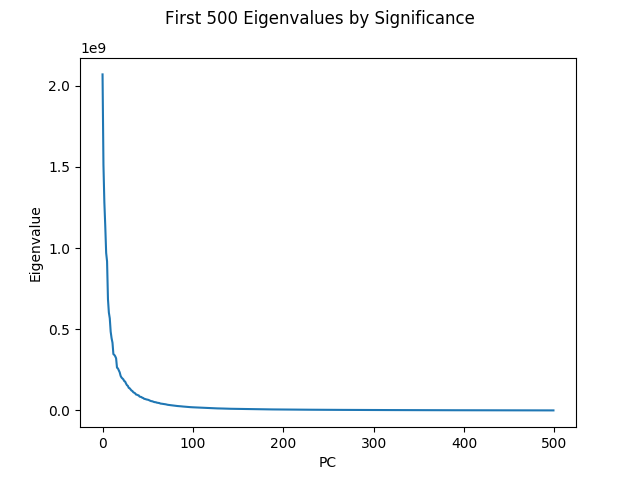
\includegraphics[scale=0.5]{hw5/Pics/2_1.png}
    \newline
    Cumulative proportion of variance explained: \newline
    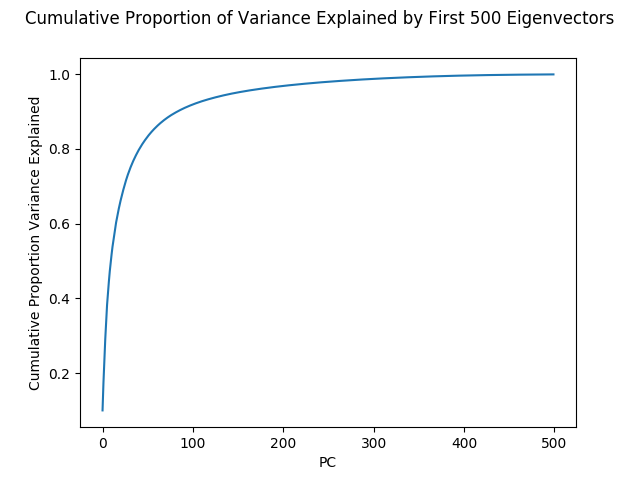
\includegraphics[scale=0.5]{hw5/Pics/2_1_2.png}
    \newline
    
    Variance explained by first 500 components: 20603735864.272518

    The cumulative proportion of variance increases rapidly until about 90-100 principle components. At that point it reaches around 0.85 of the variance and begins to increase slower. It then asymptotically approaches 1, accounting for most of the variance at about 350 principle components. So as $k$ increases so does the amount of variance explained. 
    
    \item
    Mean image:\newline
    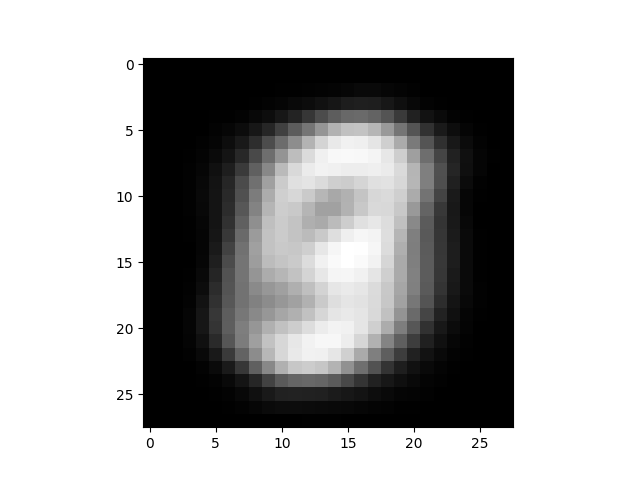
\includegraphics[scale=0.35]{hw5/Pics/2_2.png}
    \newline
    Images for first 10 principle components:\newline        \centerline{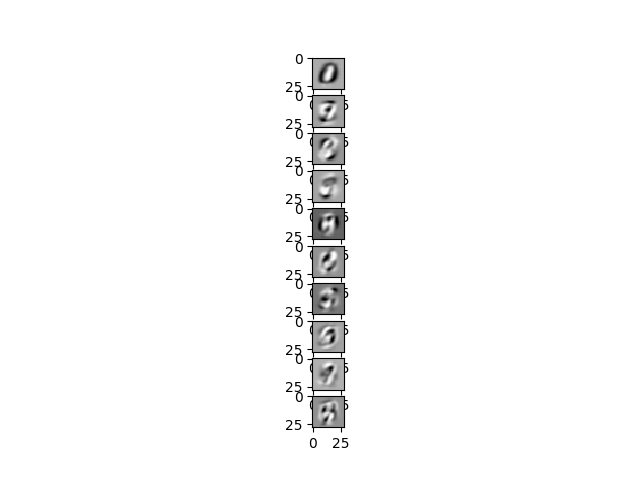
\includegraphics[scale=1.5]{hw5/Pics/2_2_2.png}}
    \newline
    
    The K-means cluster centers actually resemble digits while the principle components do not appear like digits at all (they actually do not resemble much). The principle clusters actually appear to be like partial overlays of multiple digits as opposed to a single digit that we find in K-means cluster images.
    
    
    And the mean of the data set just looks like a blurry image that overlays all the digits. 
    
    
    \item
    Reconstruction Error Using Mean Image: 7777920.419736
    
    Reconstruction Error Using first 10 PC: 12030152.311277

    The objective function using K-means is $1.26\times 10^{10}$. The reconstruction error using either method are orders of magnitude less than the objective function we got in K-means. This means that the both reconstructions perform better than K-means by a few orders of magnitude. This is likely due to the fact that the principle components create distinct approximations for each point while the K-means method only has 10 approximations for all points.
\end{enumerate}
\newpage

\begin{problem}[Bayesian Networks, 10 pts]

  \noindent In this problem we explore the conditional independence
  properties of a Bayesian Network.  Consider the following Bayesian
  network representing a fictitious person's activities. Each random
  variable is binary (true/false).

\begin{center}
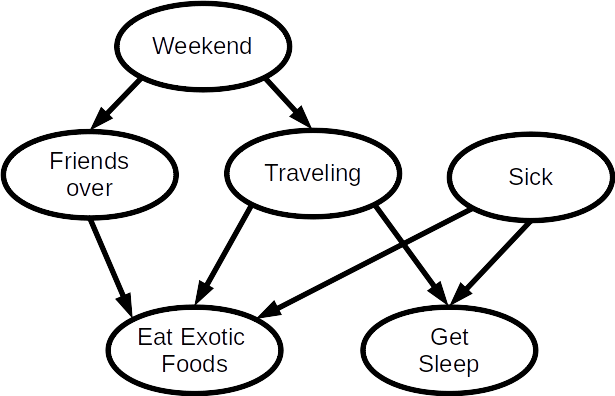
\includegraphics[width=2.5in]{bn.png}
\end{center}

The random variables are:

\begin{itemize}
\item \attr{Weekend}: Is it the weekend?
\item \attr{Friends over}: Does the person have friends over?
\item \attr{Traveling}: Is the person traveling?
\item \attr{Sick}: Is the person sick?
\item \attr{Eat exotic foods}: Is the person eating exotic foods?
\item \attr{Get Sleep}: Is the person getting sleep?
\end{itemize}

\medskip

For the following questions, $A \perp B$ means that events A and B are
independent and $A \perp B | C$ means that events A and B are independent
conditioned on C.

\textbf{Use the concept of d-separation} to answer the
questions and show your work (i.e., state what the blocking path(s) is/are and what nodes block the path; or explain why each path is not blocked).

\textbf{Example:} Is $\attr{Friends over} \perp \attr{Traveling}$? If NO, give intuition for why.

\textbf{Answer:} NO. The path from Friends over -- Weekend -- Traveling is not blocked following the d-separation rules. Thus, the two are not independent. Intuitively, this makes sense as if say we knew that the person was traveling, it would make it more likely to be the weekend. This would then make it more likely for the person to have friends over. 

\begin{enumerate}
\item Is $\attr{Sick} \perp \attr{Weekend}$?
  If NO, give intuition for why.


\item Is $\attr{Sick} \perp \attr{Friends over}\given \attr{Eat exotic
  foods}$? If NO, give intuition for why.


\item Is $\attr{Friends over} \perp \attr{Get Sleep}$? If NO, give
  intuition for why.

\item Is $\attr{Friends over} \perp \attr{Get Sleep} \given
  \attr{Traveling}$? If NO, give intuition for why.

\item Suppose the person stops traveling in ways that affect their
  sleep patterns (as various famous people have done).  Travel still
  affects whether they eat exotic foods.  Draw the modified network.

\item For this modified network, is $\attr{Friends over} \perp
  \attr{Get Sleep}$? If NO, give an intuition why.  If YES,
  describe what observations (if any) would cause them to no longer be
  independent.

\end{enumerate}
\end{problem}

\newpage
\section*{Solution}
\begin{enumerate}
    \item YES. This is true. This is because there are no active paths between the two nodes. So they must be independent in this case
    
    \item NO. This is false. In this case observing Eat exotic foods induces a correlation, effectively unblocking. Thus there is a conditional dependence between Friends over and Sick. The intuition here is that if we knew that someone ate exotic foods and observed that they have had friends over in the most likely case we know that the person is likely not sick. Since having friends over while you are sick is not likely.
    
    \item NO. This is false. Given this structure the flow of information is unblocked from Friends over to Get sleep. This goes from Friends over to Weekend to Traveling to Get sleep. The intuition here is that if we observe Get sleep we then have some information on whether it is the Weekend and subsequently some information about Friends over
    
    \item YES. This is true. By observing Traveling we block the path from Get sleep and Friends over. Due to this we have independence.   
    
    \item \hspace{2cm} \newline
    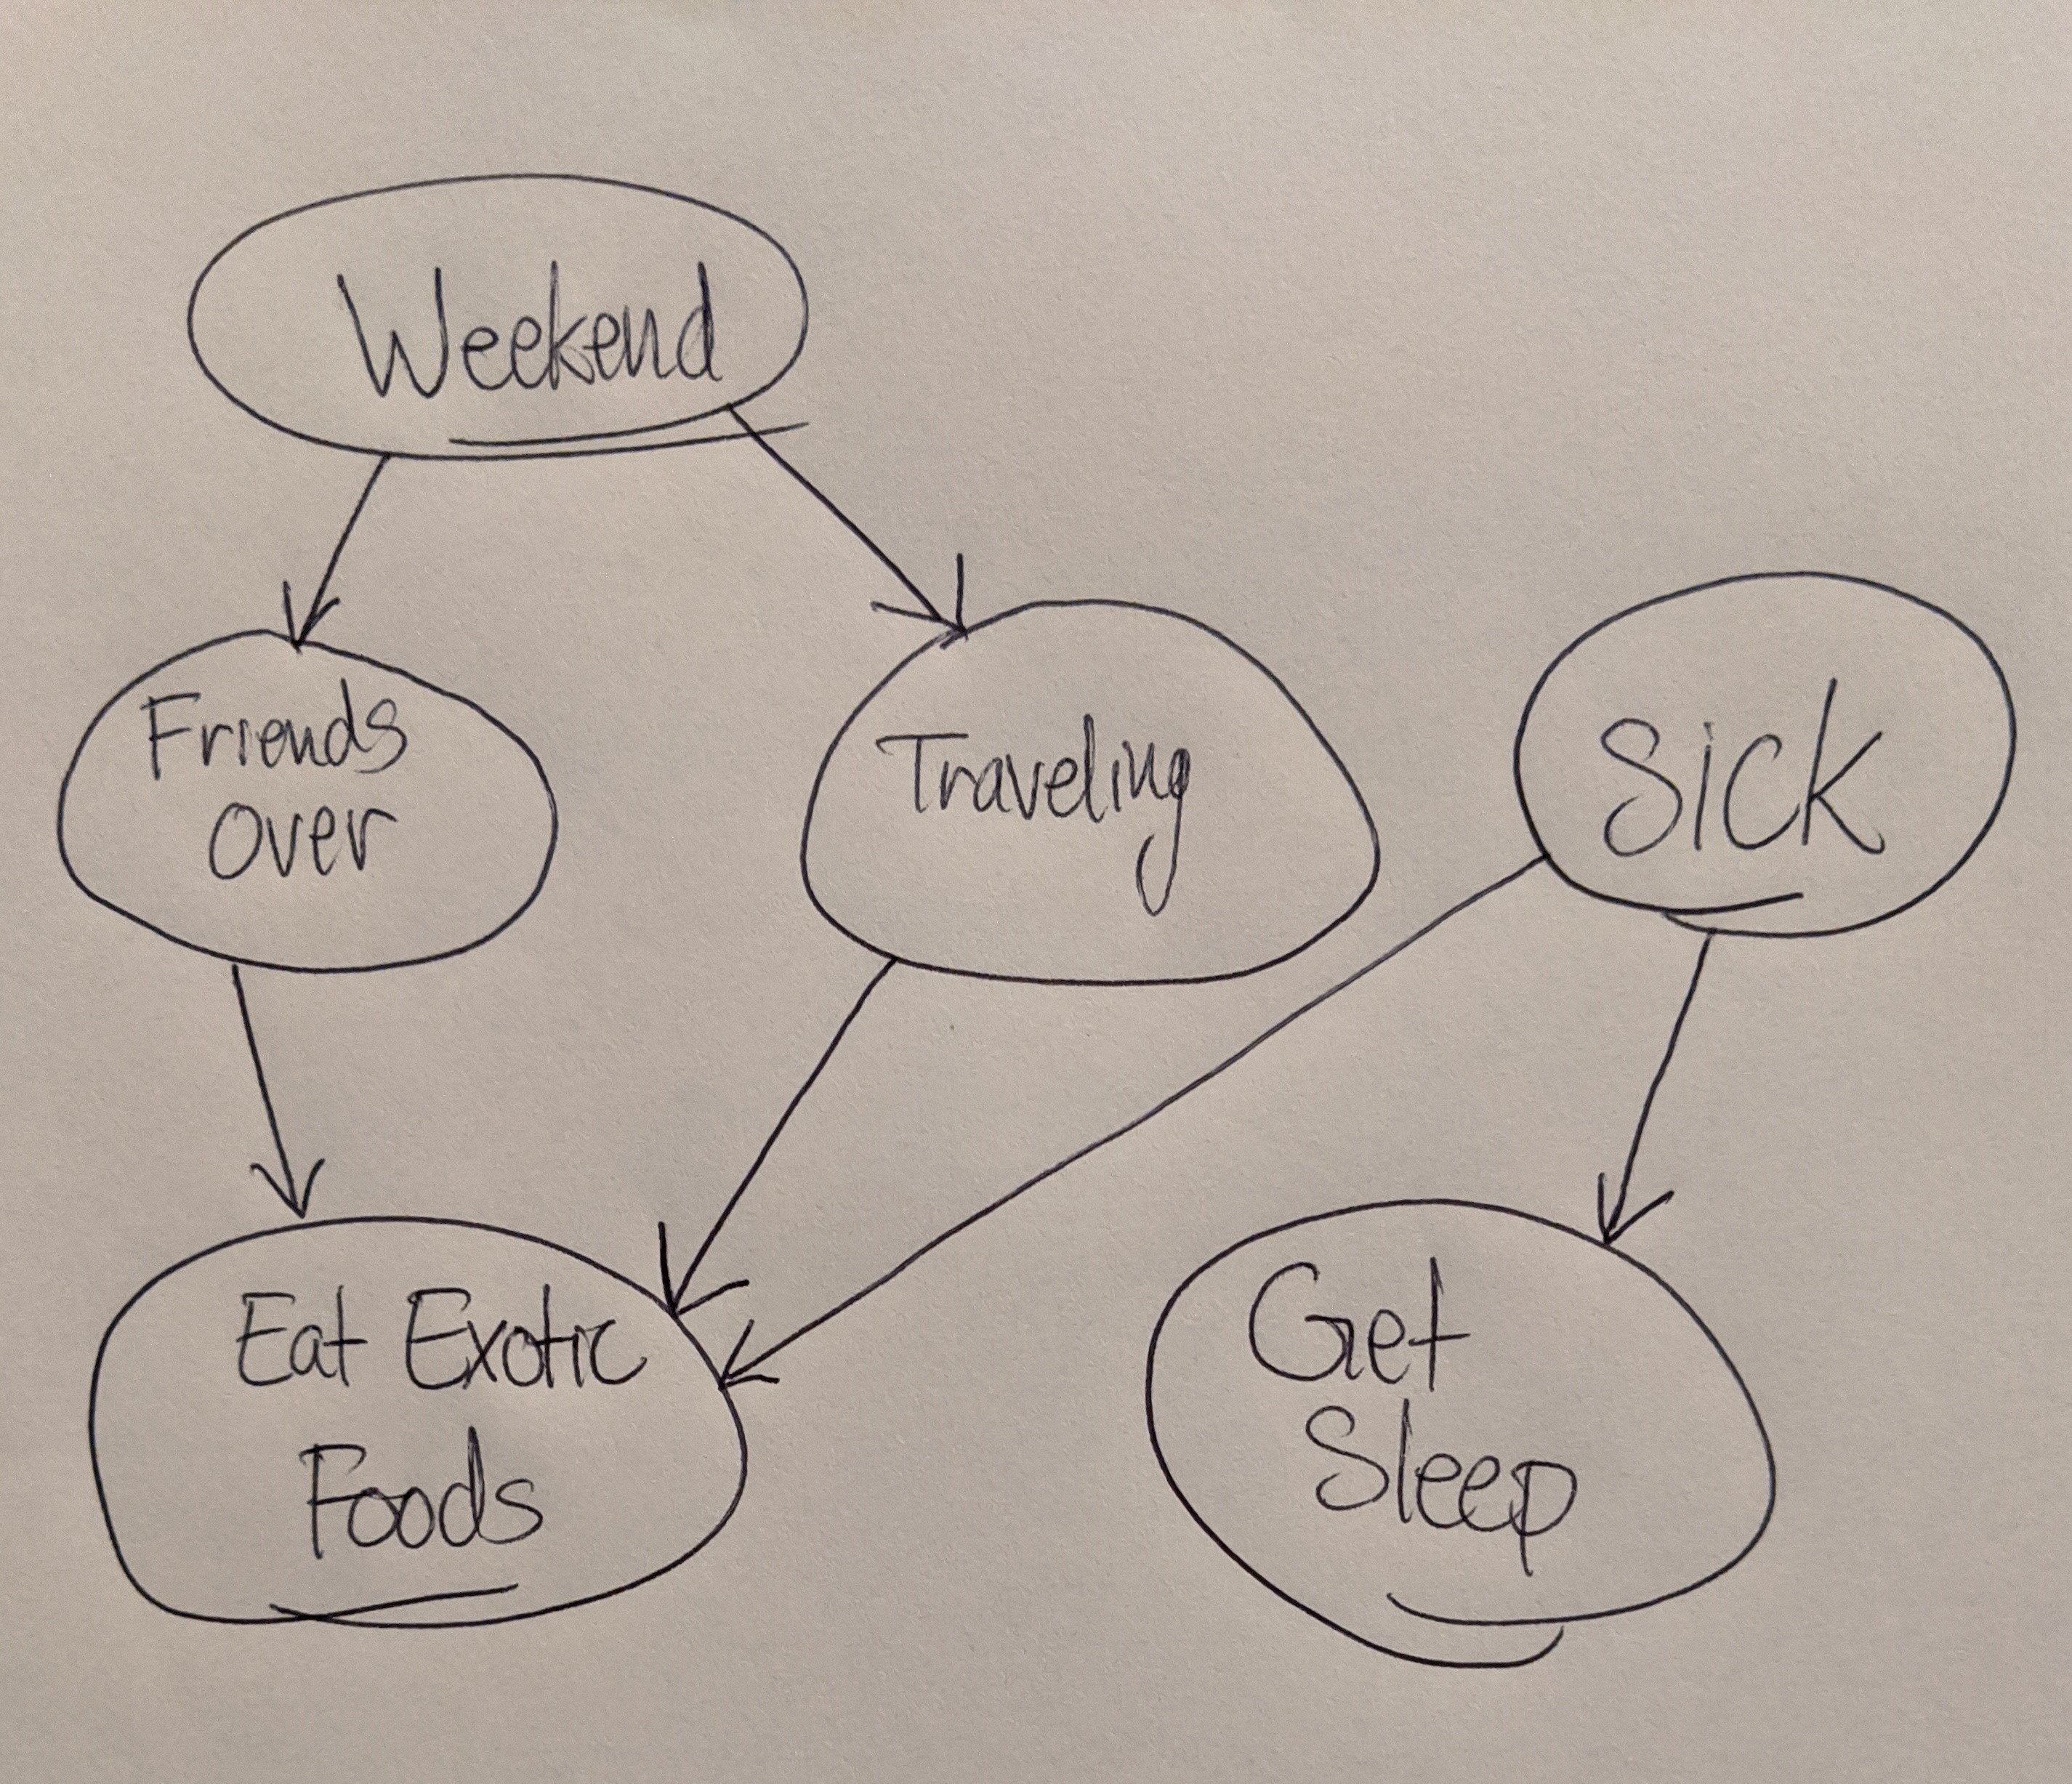
\includegraphics[width=2.5in]{hw5/Pics/network.jpg}
    
    \item YES. They are independent. If we observed Eat exotic foods we will unblock the flow of information resulting in conditional dependence.
    
\end{enumerate}

\newpage
%%%%%%%%%%%%%%%%%%%%%%%%%%%%%%%%%%%%%%%%%%%%%
% Name and Calibration
%%%%%%%%%%%%%%%%%%%%%%%%%%%%%%%%%%%%%%%%%%%%%
\subsection*{Name}

Jason Sibrian

\subsection*{Collaborators and Resources}
Whom did you work with, and did you use any resources beyond cs181-textbook and your notes?

N/A, Stack Overflow + Medium + Wikipedia (all for PCA)

\subsection*{Calibration}
Approximately how long did this homework take you to complete (in hours)? 

24

\end{document}
